\documentclass[11pt, english]{article}              
        \usepackage{geometry}
                \geometry{                          
                        a4paper,total={210mm,297mm},
                        tmargin=40.8mm,
                        bmargin=40.8mm,
                        lmargin=32.6mm,
                        rmargin=32.6mm,
                }

        \usepackage{titlesec}         
                \titleformat{\section}
                        {\normalfont\fontsize{18}{16}\bfseries}{\thesection}{0.5em}{}
                \titleformat{\subsection}
                        {\normalfont\fontsize{14}{16}\bfseries}{\thesubsection}{1em}{}
                \titleformat{\subsubsection}
                        {\normalfont\fontsize{11}{16}\bfseries}{\thesubsubsection}{1em}{}

        \usepackage{longtable}
        \usepackage{multirow}

        \usepackage[labelfont=bf,textfont=bf,font=small,skip=8pt]{caption}

        \setlength{\parindent}{0pt}
        \renewcommand{\baselinestretch}{1.25}
       \usepackage{setspace}

        \usepackage{amsmath}
        \usepackage{amssymb}

        \usepackage{graphicx}

\begin{document}

\pagenumbering{gobble}

        \title{\textsc{AG312 Advanced Corporate Finance \& Financial Markets\\ Coursework Assignment}}
        \author{\textsc{Lewis Britton}}
        \date{\textsc{Academic Year 2019/2020}}
        \maketitle

\newpage

\pagenumbering{roman}

        \renewcommand{\contentsname}{Table of Contents}

        \tableofcontents

\newpage

\pagenumbering{arabic} 

\section{General Chain of Events}

	The 2008 financial crisis is an immensely vast, complex and occasionally perplexing topic. It would be unreasonable to sequentially analyse every small detail which contributed to or had effect on the crisis however, that is exactly why we must gain a strong understanding of the surface problems, causes and effects of the crisis. As complex of a topic as this is, it can be simplified into a handful of primary causes which accumulated and provided one of the most detrimental domino effects seen by the financial industry. We must look at the role of regulation issues surrounding shadow banking and methods of securitized lending. And, the chain effect through mortgage-backed securities leading to the crisis.

	\subsection{Deregulation \& Shadow Banking}

	The first contributor is argued to be change of regulation or, deregulation in the financial industry. In 1999, there was a new act applied to replace the Glass-Steagall Act of 1933, this was known as the Gramm-Leach-Bliley Act or otherwise, as the Financial Services Modernisation Act. Traditionally, the Glass-Steagall Act deprived banks of the ability to engage in the exchange of securities (Kroszner, Rajan, 1994). Meaning there would be a clear distinction in activity between commercial and investment banks. Seen where investment banks would handle initial stock trading, primarily IPOs here, and mergers/acquisitions etc. On the other hand, commercial banks would refrain from crossing boundaries into the investment bank territory, managing checking accounts and deposits etc. Simply, investment banking could be seen as risky trading and commercial banking, far less so. This was seen in practice where, only roughly ten percent of retail banks’ income came from security trading (Maues, 2013). The passing of the Gramm-Leach-Bliley Act however, completely altered the nature of this. It allowed banks to engage in, what at the time was seen as, little to no risk derivative exchanges (Mamun, Hassan, Maroney, 2005). When combined with the role of shadow banking, there was risky engagement in security trading with hedge funds etc., as will be explored. On top of this, banks were permitted to use their own deposits to do this. 

	\subsection{Mortgage-Backed Securities}

	Banks began mortgage-backed securitizing lending at this point, which is a huge contributory factor in the mismatch of assets and liabilities (Baklanova, Copeland, McCaughrin, 2015). That is, where banks lend longer term than they borrow. Reflected where banks began to secure their investments with mortgages delivering huge risk in this market (Ashcraft, 2008). These became known as mortgage-backed securities and would be sold to a hedge fund, as with any other security. The hedge fund would then organise the mortgages using a ranking algorithm based upon factors such as the riskiness/likelihood of the mortgage taker repaying, the total sum of the mortgage owed and the value of the monthly payments (Amadeo, 2019). The hedge fund would proceed to sell the mortgage package to a cash investor. However returning to the bank, they would now make new credit card/mortgage loans based on this. This is where asset-liability mismatch can be explored further. Not only are the banks making thirty-year mortgage loans, based on shorter-term loans from other financial bodies, they also no longer officially have the mortgages in their possession.

	\subsection{Investors \& Credit Default Swaps}

	At this point in the process, the banks and hedge funds thought of themselves as extremely low risk. The cash investors on the other hand, carried heavy weight of risk on their shoulders. This is when investors were beginning to take out insurance-like instruments called Credit Default Swaps (CDSs) which protected them against the risk of default surrounding the mortgages in question (Amadeo, 2019). These act as insurance which the seller pays out, after a series of quarterly payments, in the case of default. This sense of safety simply encouraged more and more investors to purchase these mortgage-backed. This simply encouraged the banks to offer more mortgages and further dig into the idea of lending longer term than they borrow. The whole market around CDSs became very hot here. Due to the asset-liability imbalance, they were extremely volatile for the insurance companies who were issuing them. As indeed, there was very high probability of the buyers resulting in a severe case of default therefore, debt owed not being completely covered by the CDS value. That is, volumetrically speaking if an extremely high number of CDS buyers experienced default at one time, the CDS issuers may not be able to cover the cost they owe. Some however, argue that the CDS market was seen to contribute advantages as it dug into complex financial paths (Stulz, 2010). It’s seen though that this was a huge contributory factor to the fall of many insurance companies and other issuers of CDSs. And, an enormous sore for the Federal Reserve upon bailout of these companies. It must also be noted additionally that CDSs were often issued in unregulated markets (Amadeo, 2019), in which the issuers found it difficult to protect themselves in alike circumstances.

	\subsection{Sub-Prime Offerings \& Collateralised Debt Obligations}

	It’s argued that the Community Reinvestment Act contributed to the crisis where it allowed banks to take advantage of risky borrowers etc. And, it’s been found that the level of enforcement of the act in banks was positively correlated to riskiness (Agarwal, Benmelech, Bergman, Seru, 2012). This act stated that banks were not allowed to discriminate against neighbourhoods in poverty etc. Due to the banks’ strong incentive to issue mortgages at this time and the high demand for them from hedge funds etc., they began to offer mortgages to people in worse-off areas and packaged these sub-prime mortgages into what we know as Collateralized Debt Obligations. This added to the already very much present risk. Demand continued to increase while the Federal Reserve lowered interest rates, encouraging more home owners which sub-prime mortgages issuance double (Amadeo,  2019). This created the real estate ‘bubble’ we know today. The demand for mortgages only continued to grow from people nearing poverty, middle class investors and standard home owners (Amadeo, 2019); likely in addition to existing investments/real estate also. Developers struggled to keep up which is an economic issue in itself. The Federal Reserve in time however, raised interest rates returning them to a more realistic rate but this would create another domino effect in the economy. The bubble burst and with deeper analysis, this becomes easier to understand.

\newpage

\section{Structural Deregulation \& Shadow Banking}

	Banks are traditionally defined as turning savings into investments for their nation’s economy. They do this while acting as the primary lending system to our citizens based on issuing deposits and turning them into loans (McCulley, 2010). This can be simplified as maturity, liquidity and quality transformation which refers to banks loaning money on a longer maturity basis than methods utilised regarding deposit collection. Initially, banks made the pledge to only engage in low-risk trading with securities such as mortgages, bonds and Treasury Bills These were regulated, reasonably safe and proved so in historic data. Historically, banks have been in a restricted position regarding security related business. The passing of the Gramm-Leach-Bliley Act however, saw the new-found ability of banks, able to engage in trading of securities with hedge funds etc. (Mamun, Hassan, Maroney, 2005).\\

	To gain further knowledge of roles in the crisis, we must understand the term “shadow banking” in order to better understand lack of regulation. There remains a debate over the precise meaning of ``shadow banking'' however, it is loosely defined as a bank-like institution which operates similarly to a traditional bank but are viewed as less strictly regulated. Shadow banks perform standard crediting procedures  however, with an array of other financial intermediaries between (Claessens, Pozsar, Ratnovski, Singh, 2012). They also operated in a manner in which collateral is re-/abnormally used, as reflected throughout the crisis (Claessens, Pozsar, Ratnovski, Singh, 2012). Thus throughout the financial crisis, the immediately apparent components highlighted by shadow banks are securitization and collateral intermediation. These provided huge systematic risk however, due to the apparent lack of respect for various aggregate financial risk factors.\\

	Recalling the statement regarding the Gramm-Leach-Bliley Act, shadow banking had far more opportunity to be relaxed in operations. However, this lack of regulation contributed to shadow banks’ systematic risk throughout collateral intermediation (Claessens, Pozsar, Ratnovski, Singh, 2012). This further led to changes to monetary and fiscal policy in response. Further policy alterations include the rethinking of security trading policy and addressing demand pressures. The impact of this risk was foreshadowed through statistical results showing a nine-year, 250\% increase in shadow bank valuation to \$65tn in 2011 (Claessens, Pozsar, Ratnovski, Singh, 2012). This was based on the securitization and collateral operations described but the pure volume of it was observed to be in response to the growing demand for cash balance intermediation (Claessens, Pozsar, Ratnovski, Singh, 2012). Traditional banks were not well enough regulated, or even ‘deregulated’ in a sense, to operate under such demand. In effect, corporations presenting these higher cash balances saw banks being insured to intermediate over double the amount of traditional banks. This systematic risk carries implications of a market-wide fall in bad times as it ties together institutions on a macroeconomic level and delivers high probability of mutual collapse based on factors such as lack of liquidity (McCully, 2007). Add to this the fact that people were unknowingly contributing to the risk of shadow banks by utilising shadow banks for everyday banking needs etc. (Appendix A.1).\\

	Let’s recall the definition of securitization. The process of securitizing is described in two sections (Jobst, 2008). It involves one financial company holding an asset on their balance sheet with a desire to remove it and thus, selling a portfolio of alike items to another financial body who then issues relative securities which pay interest to investors. This interest is based on revenue generated by the portfolio purchased (Appendix A.2). This has significant relevance where shadow banks’ lack of regulation shackles them down in their large difference in lending/borrowing maturities, meaning payment scales and volumes simply could not be met. The process of shadow banking securitization can be demonstrated initially as a reasonably strong, regimented system (Appendix A.3). To further understand the risk associated, it must be brought to attention that they operate differently to traditional banks through intermediation roles (Claessens, Pozsar, Ratnovski, Singh, 2012). Traditional-bank intermediation involves single balance sheet operations whereas, securitization is based upon a chain of multiple balance sheet movements. This means in theory that the securitization methods have more support. It is observed therefore, that securitization involves a great amount of credit risk transfer (Claessens, Pozsar, Ratnovski, Singh, 2012), giving us an insight to the whole “who’s role was that?” aspect of the crisis. Thus throughout this chain, subsequently came the idea of these financial institutions using shorter maturity borrowing (Brunnermeier, 2009). This again reflects the image of asset-liability mismatch, contributing further to inability to meet debt.\\

	Risk must go somewhere, this is where Collateralised Debt Obligations (CDOs) enter the equation. Their simple objective is to move risk. They bundle their assets into what they call ‘tranches’ which involves three tiers based on projected and historic risk (Brunnermeier, 2009). Tranches include ‘super senior’ which is first to be paid and, at the other end, the ‘equity’ tranche which is last to be paid and is therefore far more risky. This is where mortgage securitization again becomes apparent. To recall again Credit Default Swaps (CDSs), they become very useful in cases of these low-end, poorly rated bundles. This will furthermore become apparent through the securitization of sub-prime mortgages.

\newpage

\section{Securitization of Mortgages \& Federal Reserve Rates}

	\subsection{Securitizing Sub-Prime Mortgages \& Using CDOs}

	As we’ve established, mortgages are already risky as they’re far longer term maturity items than means of financing used by their issuers. However, that’s actually a supplementary point now as issue digs much deeper. If we recall discussions of mortgage packaging, we see that the demand for these was very high. Initially we know this was due to the idea of safety/security in that owning, for example, a AAA rated mortgage package brought to an institution. Note that these AAA mortgage packages were viewed as very low risk CDOs and encouraged investment and trust. Because of this we know demand for these mortgage packages became extremely high. Thus, the issuing of very low-end mortgage packages began (Brunnermeier, 2009), where banks saw an opportunity to package, for example, mortgages from lower-income, less well-off areas, into these CDOs. Recall that the demand for mortgages form these lower income households was growing (Amadeo, 2019) and in addition to this, legislation regarding discrimination towards these households had been relaxed. Especially in the case of shadow banking.\\

	Recall that investors prefer securities with short maturities (Brunnermeier, 2009), meaning they receive their payments in a shorter period. This is reflected in short-term money market funds which generally have maturities shorter than one year. Not long into the discussed process however, institutions found the incentive to live up to the demand. They would shorten maturity rates of offerings in order to entice this market demand for short maturities. This was and should have been forecasted to be a huge mistake. It is just another demonstration of maturity mismatch. Thus, defaults would prove to be a huge cost in this situation with not enough liquidity to cover their losses. It’s argued that these banks offered this short-term debt because of their increased confidence in the AAA rated mortgage packages (Stein, 2005). Therefore, we understand that many of these sort term maturity assets sold were mortgage-backed and due to the belief/trust in these, banks and other institutions saw them as a safe form of collateral. No one accounted for a default. This can be explored further through issuing of Off-Balance Sheet Entities (OBSEs).

	\subsection{Off-Balance Sheet Entities \& Mortgage Portfolios}

	At this point, it is important to note that shadow banks were dominating over 50\% the United States (Appendix A.4) and remained `insufficiently regulated' (Valckx, 2014). This was immense compared to the UK’s far more stable rate of ten per cent. It is important to keep this idea in mind when considering OBSEs’ contribution to the financial crisis. The Basel I accord is an agreement between international financial bodies which controls guidelines surrounding banking regulation (Brunnermeier, 2009). It states that there must be a `capital charge' held by a bank at all times, more simply known as a capital requirement sitting at eight per cent. That is, at least eight per cent of the loans on banks’ balance sheets should be covered by retained capital. Banks who were holding these AAA rated mortgage packages viewed their regulatory position as an opportunity to, in a sense, reduce this capital requirement by shifting loans into what we call Off-Balance Sheet Entities (OBSEs) (Acharya, Richardson, 2009) and therefore, confirming a secure credit source through the backup of their AAA mortgage packages which are held on their balance sheet. A popular OBSE was a Structured Investment Vehicle (SIV) which was widely used to assist banks in avoiding the obligation to retain capital which covers their mortgage packages (Acharya, Richardson, 2009). Again, we see that there was clearly a sense of false safety where banks believed in these mortgage packages so much that they would attempt to transfer huge risk to them in relative cases of default. This has a double domino effect too. Not only, in the case of AAA package default would banks owe huge amounts of debt, they would have likely been lacking the funds to support such cases due to the capital requirement avoidance.\\

	The Basel II accord attempted to amend this issue by introducing charges based upon the rating of these mortgage bundles however, the OBSEs remained in aid of the banks. In effect, many sub-prime groups of mortgage packages began to receive rating which were far too generous due to the false idea of increased security through the Basel II accordance where banks were thought to be producing sufficient capital. This led to the packaging of sub-prime mortgages in tranche ratings which were above their standard. Thus, the traches closer to and including AAA were still thought of as just as safe by outside investors however, were much more prone to default. This is seen to have great impact where banks continued to use these to `securely' back the loans they were making. In turn, leading to larger scale and scope of defaults and thus, greater maturity/asset-liability mismatch.\\
	
	Banks managed to create what was viewed as a risk-free environment by implementing Asset Backed Commercial Papers (ABCPs), which are a form of OBSE (Acharya, Schnabl, 2010). In effect, these aided banks in their purchasing of long term debt while lending on a short term basis. Where ABCPs were at one point reported to have an average maturity of four days (Covitz, Liang, Suarez, 2009), whilst banks remained investing in long-term debt. Of course, this simply made it easier for banks to lend/spend as people continued to have belief in the AAA, or alike, mortgage packages being a secure enough mean of `back-up'. This is reflected in the extreme, almost one hundred percent, increase in outstanding ABCPs leading up to the start of the crisis in 2007 (Appendix A.5). Banks were using these `supportive' assets to fund long-term debt and remained issuing shorter-term debt, while they continued to package the sub-prime mortgages in these upper tranches. Thus, enhancing the default effect of mortgages on subsequent financial bodies etc. We see a downturn in ABCPs after 2007 (Appendix A.5) where people were establishing the scale of how uncertain ABCPs actually were. And so, not only were these ABCPs able to assist banks in the crisis, they were also receiving less investment in them. In short, banks would buy long-term debt funded by short-term maturity issuing of ABCPs. Thus, the investors were risk-averse but lacked knowledge. The risk appears to be covered by the AAA mortgage packages but banks were to blind to realise the risk in these. Hence, chain default. Once again showing us the issue is an unbelievably naïve maturity mismatch. Thankfully in time, the Financial Reporting Consolidation (FIN 46) regulated OBSEs and ceased banks from issuing them (Covitz, Liang, Suarez, 2009). However, this did also contribute to the crisis in the sense that banks no longer had the option to raise funds through this very profitable method.

	\subsection{CDS Issuance \& Fall of Issuers}

	Throughout the process of firms investing in any of the discussed mortgage portfolios or indeed, any other alike portfolios/assets, institutions would frequently take out Credit Default Swaps (CDSs) which in this case acted as their insurance against the risk within the Off-Balance Sheet Entity process (Brunnermeier, 2009). These were issued by firms such as the American International Group. In this situation, the Lehman Brothers gain their recognition as they were a well-known purchaser of CDSs. In this specific scenario, CDSs purchased by the Lehman Brothers acted as their insurance against default of their mortgages portfolios. Corporations with a Collateralised Debt Obligation of AAA mortgages and CDSs were viewed as very low risk (Brunnermeier, 2009). This was due to the likelihood of AAA related default being thought to be very low and therefore, for the CDS issuer – to this package owner – being thought to be of low risk. Recall from previous discussions, the idea of banks offering shorter term debt while investing in longer term debt – a maturity mismatch – due to their belief in themselves and investors’ belief in them. CDSs also add a huge degree of confidence to this situation and give investors peace of mind. In this case, false peace of mind. Investors may only be investing in short term debt with the banks in question however, the huge risk factor remains.\\

	Throughout the period of the crisis in 2007, it is estimated that outstanding CDS value ranges from \$45tn to \$62tn (Brunnermeier, 2009). And thus, the valuation of mortgage Credit Default Swaps dropped drastically form July 2007 (Appendix A.6). Seeing that the sub-prime BBB- packages ended up in the worse-off position, well below AAA in the end – which still saw an immense sixty percent drop from this point in 2007. These statistics simply demonstrate to us that the idea of CDSs and related default in mortgages, thus banks and all the others in between, can be applied to any of the previously discussed situations. This therefore, leaves not only the home owner, the banks and other intermediaries in debt/huge risk of closure; it leaves the CDS issuers in a very, sometimes undeserving, similar situation. The value of what was owed by the banks etc. could simply not be covered by the value of the CDS insurance. CDS issuers like American International Group required severe help too and in many cases, faced bankruptcy.

	\subsection{Repurchase Agreements \& The Federal Reserve}

	Banks have been using repurchase agreements, ``repos'', for many years however, they became immediately apparent during the crisis. Repos are a standard form of securitized lending where one firm sells an asset to another with a promise to buy it back at a later date, at a specified price (Gorton, G., Metrick, A. (2009); based on interest paid upon repurchase (Appendix A.7). Repos are frequent in times when firms want to raise cash urgently, as seen in the crisis. On top of this, we see that banks were executing these short-term repos in order to fund mortgage issuing, similar to OBSEs. Recall, they were still implementing the mortgage packages here: standard and the falsely ranked sub-prime. The growth of subprime mortgages and banks’ inclination to securitize these witnessed the huge increase in repo activity/value leading up to the crisis (Copeland, Martin, Walker 2014). This came with huge uncertainty however, being larger than the relative GDP at that time. This shows severe over-inflation.\\

	As we’ve established, banks continued to believe their mortgage packages, used for securitization, were low risk. Repurchase agreements are afterall, based on the absence of risk. However, banks became over-reliant on these short-term repos and thus when the downturn began, reliance on repo peaked at 32\% of total liabilities (Appendix A.8). This is once again also a case of maturity mismatch. Banks were financing long-term mortgages with short-term debt. In a case of default, we see a repeat of the previously discussed and alike outcomes. We know that at this point, most of the risk was lying with the banks. Even if they didn’t believe it. This means many financial bodies required their stability. We know through mortgage default that this aided the collapse. Note that the degree to which a loan is over collateralised is called the “haircut” (Baklanova, Copeland, McCaughrin, 2015). And so, banks began to realise that their securitization was riskier than they thought and people began to demand their money back urgently but if we recall their maturity mismatch, we know that they don’t have the funding/ability as it is lent long-term somewhere else. Thus, we observe just about everyone selling their collateral at once leading to a `fire sale'. It is argued that this could have been avoided by altering the haircuts of a repo relative to the risk (Baklanova, Copeland, McCaughrin, 2015). Making it fairer to investors and reducing panic in the realisation of riskiness. But, all of the collateral ended up on the market at once which led to a fall in prices primarily as there was a lack of buyers due to these trust issues. If the investors simply accepted the risk at an adjusted haircut, it’s argued that there wouldn’t have been a crisis. Perhaps just a decline.\\

	This situation has become more regulated since the crisis however. In 2011, the Federal deposit Insurance Corporation extended assessments to all of banks’ liabilities which in turn made it more expensive for banks to engage in repo-based borrowing (Baklanova, Copeland, McCaughrin, 2015). This was aided by an additional rule in the Basel III agreement where banks were vigorously encouraged to extend the maturities of their borrowing. In effect, the repo market has been stabilised in a sense since the crisis. It has been argued though that some previous change in regulation contributed to the crisis. When the repo rate was raised, the Federal Reserve had a lot of cash and therefore, should be injecting it into the falling repo market. However, the changing legislation required them to retain rather than such, meaning this issue was added on top of the already apparent maturity mismatch.\\

\newpage

\section{Conclusions}

	We see here that the 2007/2008 financial crisis is a deep and complex road to venture down. Hence, the underregulated and uncertainty surrounding the shadow banking industry allowed for more financial exploits than the economy could handle. The passing of new and arguably ‘relaxed’ pieces of legislation, such as the Gramm-Leach-Bliley Act, added to the expandability and investment opportunities for banks – now able to engage in security trading with hedge funds etc. At this point, banks began engaging in Collateralized Debt Obligation compilation of mortgage packages, including falsely ranked sub-prime mortgages; in cases used to fund more long-term debt, leading to maturity mismatch based on the banks’ short-term financing methods. These mortgage packages appeared safe to risk-averse investors who, along with banks, did not realise the default risk involved with them due to apparent `safe' labelling. AAA etc. To protect themselves, banks engaged in CDS purchasing which insured them in cases of default. Little did they expect however, for great amounts of default to coincide and for CDS issuers such as American International Group to struggle to cover insurance costs. Hence, default also effected banks from the previously explored aspect of maturity mismatch as they lacked liquid funds. Hence, banks and insurance issuers, and plenty of other financial bodies collapsed in result.\\

	In addition to this, banks engaged in OBSE issuance which was theorised to transfer risk. However as was observed, banks simply piled on to their asset-liability mismatch with this fund-raising method, with inability to cover costs in default cases. Alike situations involving CDSs repeated here. Similar cases were demonstrated through repurchase agreements and securitized lending where banks were far too greedy in demanding investment rather than satisfying investors. Observed through the haircut issue etc. Thus again, it all reduces to the maturity/asset-liability mismatch in banks overconfident and greedy nature. Security lenders are a central reliance and things fall when they do. Hence, the chain downfall. Legislation has been passed since which makes the system and issuance of such `home-made' assets more intangible, such as the Basel III agreement and FIN 46. It simply would have been a beneficial idea for a higher and more knowledgeable body than greedy cash-centric-minded banks to be calling the final shots on such risky occasions.

\newpage

\section*{Appendices}

	\subsection*{Appendix 1: Figures \& Models}

	\textbf{A.1: Addition of Non-Mortgage Backed Securities}

	\begin{center}
		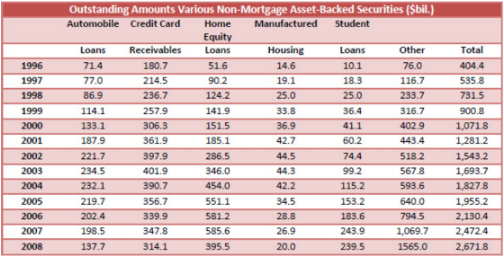
\includegraphics[height=4.5cm,width=8cm]{AG312-IMG/a.png}
	\end{center}

	\textbf{A.2: What is Securitization?}

        \begin{center}
                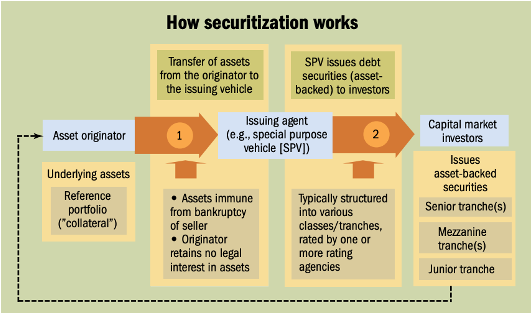
\includegraphics[height=5cm,width=9cm]{AG312-IMG/b.png}
        \end{center}

	\textbf{A.3: Shadow Banks \& Securitization}

        \begin{center}
                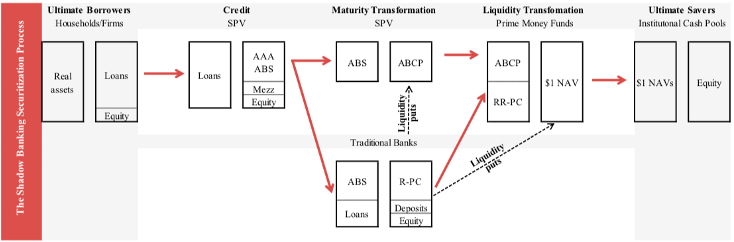
\includegraphics[height=4.5cm,width=12cm]{AG312-IMG/c.png}
        \end{center}

\newpage

        \textbf{A.4: Shadow Bank Scale}

        \begin{center}
                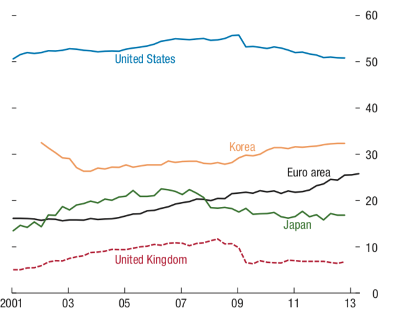
\includegraphics[height=5cm,width=6cm]{AG312-IMG/d.png}
        \end{center}

	\textbf{A.5: Asset Backed Commercial Paper}

        \begin{center}
                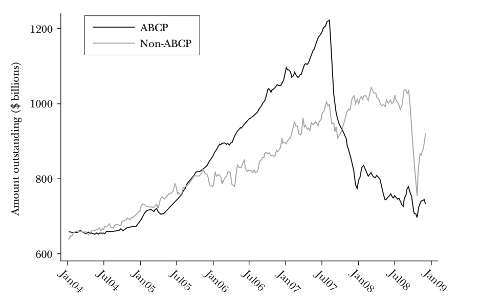
\includegraphics[height=5cm,width=7cm]{AG312-IMG/e.png}
        \end{center}

        \textbf{A.6: Mortgage CDO Value}

        \begin{center}
                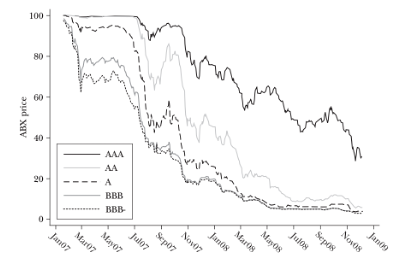
\includegraphics[height=5cm,width=7cm]{AG312-IMG/f.png}
        \end{center}

\newpage

        \textbf{A.7: General Bilateral Repurchase Agreement}

        \begin{center}
                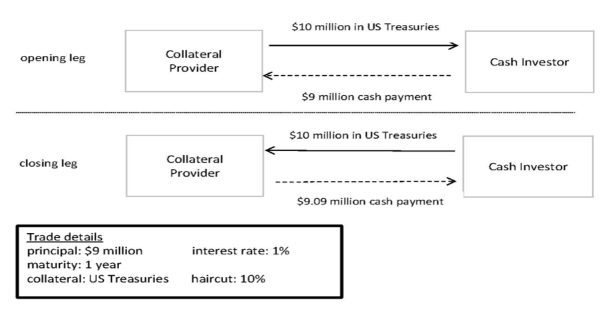
\includegraphics[height=6.5cm,width=12cm]{AG312-IMG/g.png}
        \end{center}

	\textbf{A.8: Repo Liabilities as a Percentage of Total Liabilities}

        \begin{center}
                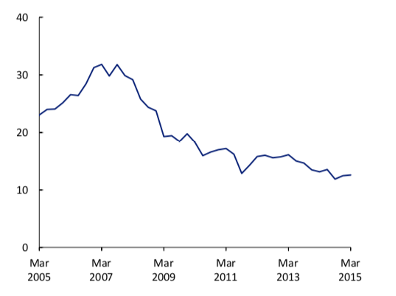
\includegraphics[height=5cm,width=6cm]{AG312-IMG/h.png}
        \end{center}

\newpage

\renewcommand\refname{Bibliography}

\begin{thebibliography}{9}

	\bibitem{a}
		Acharya, V., Richardson, M. (2009).
		\textsl{Causes of the Financial Crisis.}
		Critical Review.

	\bibitem{b}
		Acharya, V., Schnabl, P. (2010).
		\textsl{Do Global Banks Spread Global Imbalances? Asset-Backed Commercial Paper During the Financial Crisis of 2007-09.}
		IMF Economic Review.
                 
	\bibitem{c}
		Agarwal, S., Benmelech, E., Bergman, N., Seru, A. (2012).
		\textsl{Did the Community Reinvestment Act (CRA) Lead to Risky Lending?}
		National Bureau of Economic Research.
                
	\bibitem{d}
		Amadeo, K. (2019).
		\textsl{Causes of the 2008 Financial Crisis.}
		Available At:
		\texttt{https://www.thebalance.com/what-caused-2008-global-financial-crisis-3306176}
                     
        \bibitem{e}  
		Ashcraft, A. (2008).
		\textsl{Understanding the Securitization of Subprime Mortgage Credit.}
		Foundations and Trends in Finance.

        \bibitem{f}
		Baklanova, V., Copeland, A., McCaughrin, R. (2015).
		\textsl{Reference Guide to US Repo and Securities Lending Markets.}
		Office of Financial Research.
                
	\bibitem{g}
		Brunnermeier, M. (2009).
		\textsl{Deciphering the Liquidity and Credit Crunch 2007-2008.}
		Journal of Economic Perspectives.
                     
        \bibitem{h}  
		Claessens, S., Pozsar, Z., Ratnovski, L., Singh, M., (2012).
		\textsl{Shadow Banking: Economics and Policy.}
		International Monetary Fund.

        \bibitem{i}
		Copeland, A., Martin, A., Walker, M. (2014).
		\textsl{Repo Runs: Evidence from the Tri-Party Repo Market.}
		Federal Reserve Bank of New York: Staff Reports.
                
	\bibitem{j}
		Covitz, M., Liang, N., Suarez, G. (2009).
		\textsl{The Evolution of a Financial Crisis: Collapse of the Asset-Backed Commercial Paper Market.}
		Journal of Finance, Forthcoming.
                     
        \bibitem{k}  
		Gorton, G., Metrick, A. (2009).
		\textsl{Securitized Banking and the Run on Repo.}
		Yale \& NBER.

        \bibitem{l}
		Gorton, G. (2009).
		\textsl{Slapped in the Face by the Invisible Hand: Banking and the Panic of 2007.}
		Bond Market Association, Bloomberg.
                
	\bibitem{m}
		Jobst, A. (2008).
		\textsl{What Is Securitization?}
		Finance \& Development.
                     
        \bibitem{n}  
		Kroszner, R., Rajan, R. (1994).
		\textsl{Is the Glass-Steagall Act Justified? A Study of the US Experience with Universal Banking Before 1933.}
		The American Economic Review.

        \bibitem{o}
		Mamun, A., Hassan, M.K., Maroney, N. (2005).
		\textsl{The Wreath and Risk Effects of the Gramm-Leach-Bliley Act (GLBA) on the US Banking Industry.}
		Journal of Business Finance.
                
	\bibitem{p}
		Maues, J. (2013).
		\textsl{Banking Act of 1933 (Glass-Steagall).}
		Federal Reserve Bank of St. Louis.
                     
        \bibitem{q}  
		McCulley, P. (2010).
		\textsl{Before the Financial Crisis Inquiry Commission.}
		Statement of Paul A. McCulley: Managing Director, PIMCO.

        \bibitem{r}
		Stein, J. (2005).
		\textsl{Why Are Most Funds Open-End? Competition and the Limits of Arbitrage.}
		Quarterly Journal of Economics.
                
	\bibitem{s}
		Stulz, R. (2010).
		\textsl{Credit Default Swaps and the Credit Crisis.}
		Journal of Economic Perspectives.
                     
        \bibitem{t}  
		Valckx, Nico. (2014).
		\textsl{Shadow Banking Around the Globe: How Large, And How Risky?}
		International Monetary Fund.

\end{thebibliography}

\end{document}
